% vim:ft=tex:
\documentclass[debug, font=Times]{gw-dissertation}[2021/11/19]
\usepackage{lipsum}  % to generate random paragraphs
\usepackage[none]{hyphenat}  % disable hyphenation; not required by GW guideline
\sloppy  % to make long but non-hyphenated words go to the next line

% configuration for front pages (commands came from gw-dissertation class)
\title{Example Dissertation}
\author{First Last}
\defdate{Spring 2022}
\gradyear{2022}
\gradmonth{05}
\graddate{31}
\advisor{First Last}{Professor of Sadness Engineering}
\school{School of Life Destroying}
\dedication{\lipsum[2-3]}
\acknowledgments{\lipsum[2-3]}
\disclaimer{\lipsum[2-3]}
\abstract{\lipsum[2-3]}
\preface{\lipsum[2-3]}
\prevdegree{B.A. in Happiness Engineering, May 2006, University of Happy Valley}
\prevdegree{M.S. in Happiness Engineering, January 2008, University of I don't remember}
\committee{First1 Last1, Professor of Sadness Engineering, Dissertation Director}
\committee{First2 Last2, Professor of Sadness Engineering, Committee Member}
\committee{First3 Last3, Professor of Sadness Engineering, Committee Member}
\committee{First4 Last4, Professor of Sadness Engineering, Committee Member}

% other configurations
\addbibresource{reference.bib}  % bib file location
\graphicspath{{figs}}  % default path to search for figures

% begin the dissertation
\begin{document}

\chapter{Introduction}

Start each chapter on a new page. All of the text on this page starts at the same location on the
ruler bar except for the first line of text of each new paragraph.

Note that each level is indented in a $1/4$ inch (or two dots to the right on the ruler bar) from
the last section header. 

    \section{Second Level Header}
    Start your text here.

    \section{Second Level Header}
    Start your text here.

        \subsection{Third Level Header}
        Start your text here.

            \subsubsection{Fourth Level Header}
            Start your text here.

                \paragraph{Fifth Level Header}
                Start your text here.

\chapter{Literature Review or Your Heading}

Start your text and double-space the text.
\begin{figure}[h!]
    \Centering
    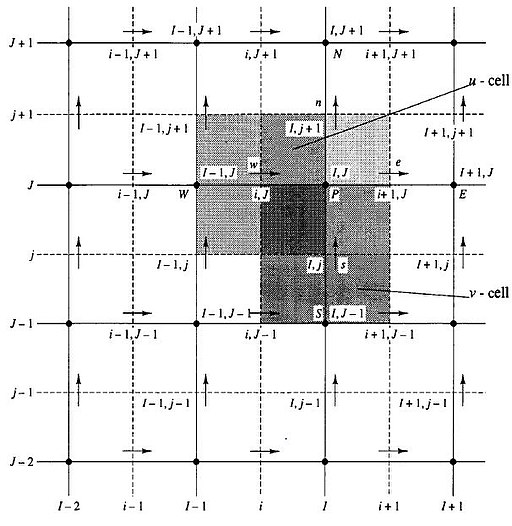
\includegraphics[width=0.5\linewidth]{grid.jpg}
    \caption{Staggered grid (public domain figure)}
\end{figure}
\begin{figure}[h!]
    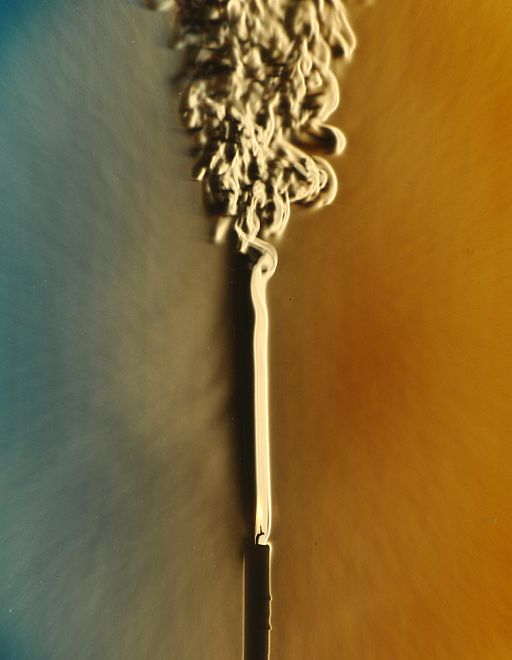
\includegraphics{laminar_turbulent_transition.jpg}
    \caption{%
        Laminar turbulent transition (public domain figure). I am trying to make the cpation%
        longer so that we can see how this class handle long captions. I am trying to make the %
        cpation longer so that we can see how this class handle long captions.%
    }
\end{figure}

\chapter{Methods or Your Heading}

Start your text and double-space the text.
\begin{figure}[h!]
    \Centering
    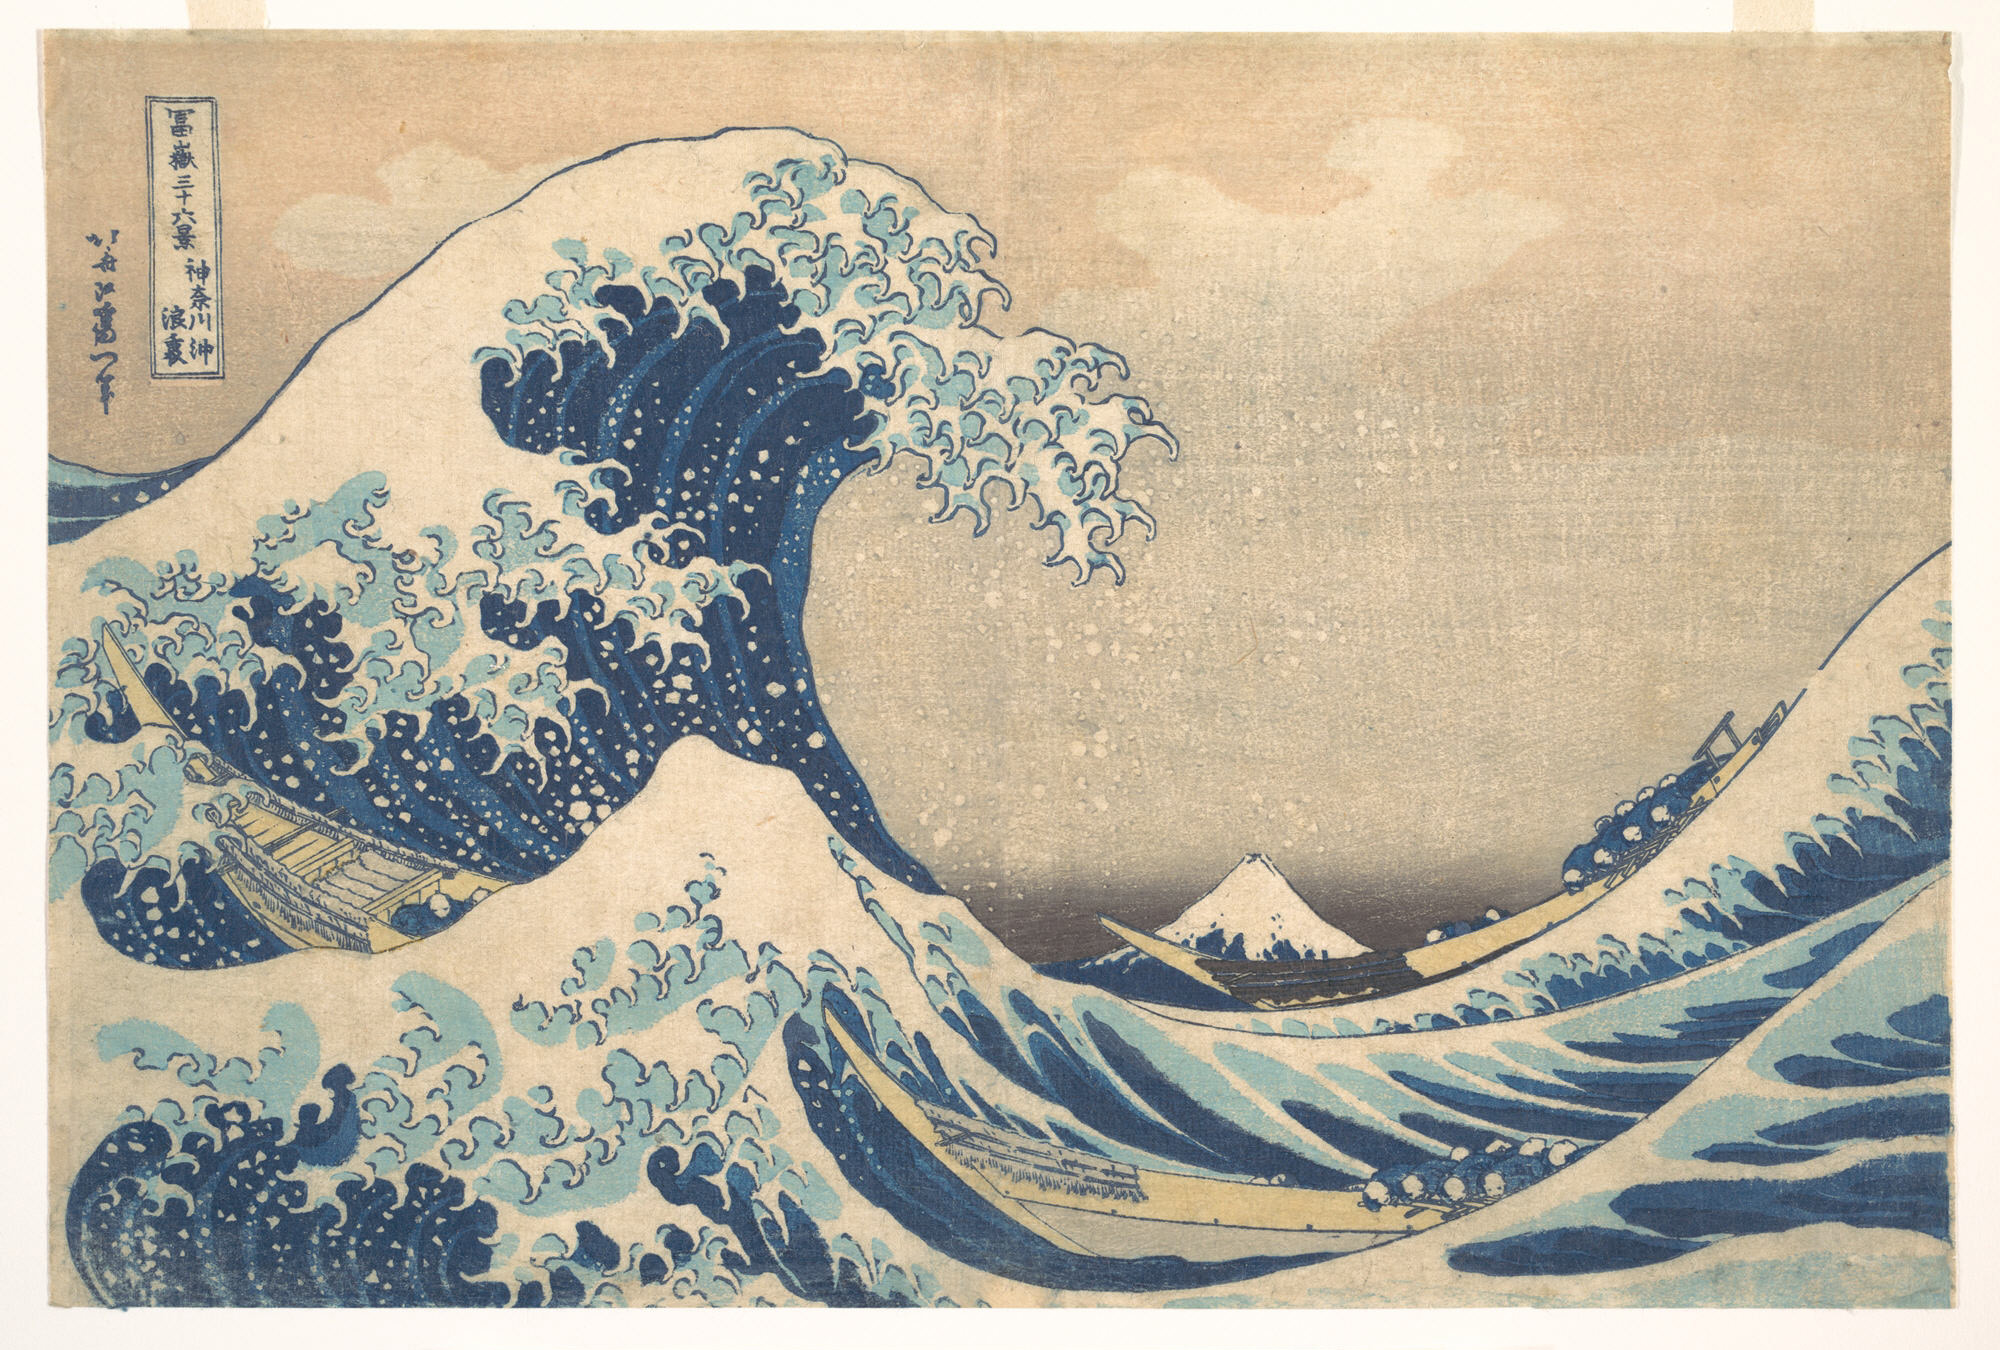
\includegraphics[width=0.5\linewidth]{the_great_wave.jpg}
    \caption{The Great Wave off Kanagawa by Katsushika Hokusai (public domain figure)}
\end{figure}

\chapter{Results or Your Heading}

Start your text and double-space the text.
\begin{table}[h!]
    \Centering
    \begin{tabular}{||c c c c||}
         \hline
         Col1 & Col2 & Col2 & Col3 \\ [0.5ex]
         \hline\hline
         1 & 6 & 87837 & 787 \\
         2 & 7 & 78 & 5415 \\
         3 & 545 & 778 & 7507 \\
         4 & 545 & 18744 & 7560 \\
         5 & 88 & 788 & 6344 \\ [1ex]
         \hline
    \end{tabular}
    \caption{Example table 1}
\end{table}

\chapter{Discussion, Conclusion, or Your Heading}

Start your text and double-space the text. This is a fake citation \cite{author1_1990}. This is
another fake citation \cite{author2_2000}.
\begin{table}[h!]
    \Centering
    \begin{tabular}{||c c c c||}
         \hline
         Col1 & Col2 & Col2 & Col3 \\ [0.5ex]
         \hline\hline
         1 & 6 & 87837 & 787 \\
         2 & 7 & 78 & 5415 \\
         3 & 545 & 778 & 7507 \\
         4 & 545 & 18744 & 7560 \\
         5 & 88 & 788 & 6344 \\ [1ex]
         \hline
    \end{tabular}
    \caption{Example table 2}
\end{table}

\sloppy
\printbibliography
\fussy

\appendix
\chapter{The Heading of Appendix A}

    \section{Appendix Can Have Sections}
    Start your text here and double- space the text.
    \begin{figure}[h!]
        \Centering
        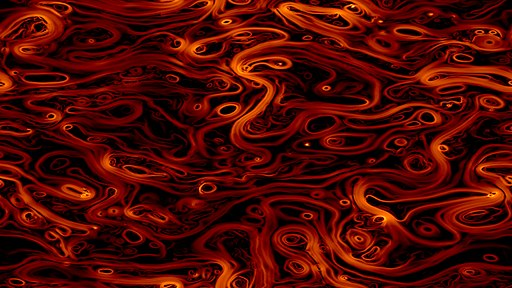
\includegraphics[width=0.5\linewidth]{magnetic_turbulence.jpg}
        \caption{Magnetic turbulence (public domain figure)}
    \end{figure}

        \subsection{Appendix Can Have Subsections}
        Start your text here and double- space the text.
        \begin{figure}[h!]
            \Centering
            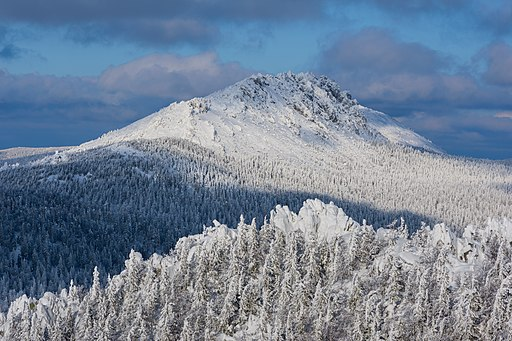
\includegraphics[width=0.5\linewidth]{mt_otkliknoy_greben.jpg}
            \caption{Mt. Otkliknoy Greben (public domain figure)}
        \end{figure}

    \section{Appendix Can Have Sections}
    Start your text here and double- space the text.

\chapter{The Heading of Appendix B}
Start your text here and double- space the text.
\begin{table}[h!]
    \Centering
    \begin{tabular}{||c c c c||}
         \hline
         Col1 & Col2 & Col2 & Col3 \\ [0.5ex]
         \hline\hline
         1 & 6 & 87837 & 787 \\
         2 & 7 & 78 & 5415 \\
         3 & 545 & 778 & 7507 \\
         4 & 545 & 18744 & 7560 \\
         5 & 88 & 788 & 6344 \\ [1ex]
         \hline
    \end{tabular}
    \caption{Example table 3}
\end{table}

\end{document}
